%%%%%%%%%%%%%%%%%%%%%%%%%%%%%%%%%%%%%%%%%%%%%%%%%%%%%%
\section{はじめに}
%%%%%%%%%%%%%%%%%%%%%%%%%%%%%%%%%%%%%%%%%%%%%%%%%%%%%%
 電離圏研究のために実施されている短波ドップラー(HFD)観測のデータはオープンデータとして公開されており,自由な使用が認められている.
現状,データ活用を促進するために数件の web アプリケーションが開発されているが,多くが開発運用の困難性やユーザーエクスペリエンス等の観点で問題を抱えている.
 この課題点を解消するため既存のアプリケーションの課題点から必要要件を洗い出し,ページレンダリング手法を考慮した web アプリケーションの新規設計を行う.本研究ではその中の web スクレイピングを用いてデータを取得する処理,および,取得したデータを整形して扱いやすくする処理に焦点を当て研究を行う.
本研究ではNext.jsと呼ばれるフレームワークを用いて実装を行う.JavaScriptのUIライブラリの一つであるReact.jsがベースとなっており,サーバ機能も有しているため効率的なweb開発が可能である.また,使用する言語を統一して管理コストの低減を図るため,webスクレイピングはTypeScriptを用いて行う.

%%%%%%%%%%%%%%%%%%%%%%%%%%%%%%%%%%%%%%%%%%%%%%%%%%%%%%
\section{Webスクレイピングについて}
%%%%%%%%%%%%%%%%%%%%%%%%%%%%%%%%%%%%%%%%%%%%%%%%%%%%%%
webスクレイピングとは,web サイトから情報を抽出するコンピュータソフトウェア技術のことを指す.HTML フォーマットからテキストを抽出してスプレッドシートや json ファイル等の構造化データへの変換を行うことができ,web 上にあるデータを取得して扱うことを目的とする.web スクレイピングの手法としては,正規表現や DOM 解析,HTML パーサ等を用いたものがある.本研究では,ISRを用いたwebアプリケーションを設計するため,スクレイピングの処理に速度を求める必要がない.そのため,本研究では軽量でサーバへの負担が小さいcheerioをHTMLパーサとして用いる.
%%%%%%%%%%%%%%%%%%%%%%%%%%%%%%%%%%%%%%%%%%%%%%%%%%%%%%
\section{使用ライブラリ}
%%%%%%%%%%%%%%%%%%%%%%%%%%%%%%%%%%%%%%%%%%%%%%%%%%%%%%
% ----- figure ---------------------------------------------------------
\begin{figure}[b!]
	\medskip
	\centering
	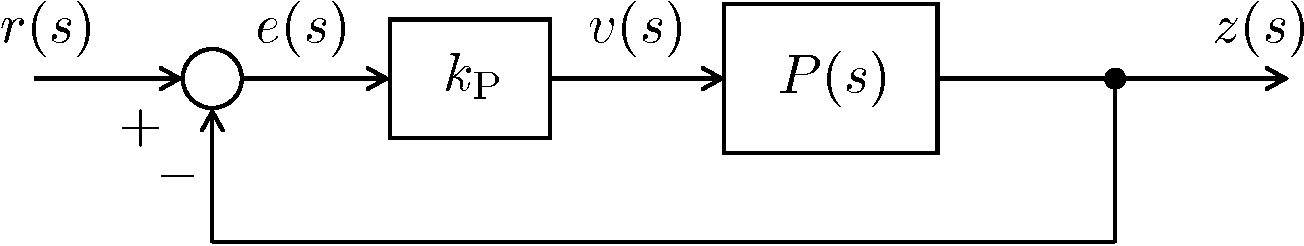
\includegraphics[scale=0.35]{fig/figure-crop.pdf}
	\caption{フィードバック制御系}
	\label{fig:feedback}
	\medskip
\end{figure}
% ----- figure ---------------------------------------------------------
% ----- figure ---------------------------------------------------------
\begin{figure}[b!]
	\medskip
	\centering
	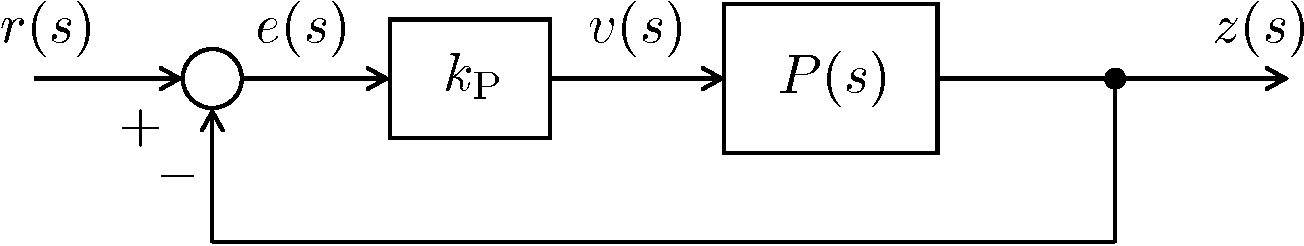
\includegraphics[scale=0.35]{fig/figure-crop.pdf}
	\caption{□□□□□□□□□□□□□□□□□□□□□□□□□}
	\label{fig:feedback2}
	\medskip
\end{figure}
% ----- figure ---------------------------------------------------------
 □□□□□□□□□□□□□□□□□□□□□□□□□□□□□□□□
□□□□□□□□□□□□□□□□□□□□□□□□□□□□□□□□□
\begin{eqnarray}
	a = b + \dfrac{\sqrt{c + 3}}{2}
\end{eqnarray}
□□□□□□□□□□□□□□□□□□□□□□□□□□□□□□□□□
□□□□□□□□□□□□□□□□□□□□□□□□□□□□□□□□□
□□□□□□□□□□□□□□□□□□□□□□□□□□□□□□□□□
□□□□□□□□□□□□□□□□□□□□□□□□□□□□□□□□□



%%%%%%%%%%%%%%%%%%%%%%%%%%%%%%%%%%%%%%%%%%%%%%%%%%%%%%
\subsubsection{□□□□□□□□□□□□□□□□□□□□□□□□□□□}
%%%%%%%%%%%%%%%%%%%%%%%%%%%%%%%%%%%%%%%%%%%%%%%%%%%%%%
 □□□□□□□□□□□□□□□□□□□□□□□□□□□□□□□□
□□□□□□□□□□□□□□□□□□□□□□□□□□□□□□□□□
□□□□□□□□□□□□□□□□□□□□□□□□□□□□□□□□□
□□□□□□□□□□□□□□□□□□□□□□□□□□□□□□□□□
% ----- table ---------------------------------------------------------
\begin{table}[t!]
	\centering
	\medskip
	\caption{限界感度法}
	\label{table:pid}
	\smallskip
	\begin{tabular}{|c|c|c|c|}
		\hline
		& ${k}_{\rm P}$ & ${T}_{\rm I}$ & ${T}_{\rm D}$ \\\hline
		P 制御   & $0.5{k}_{\rm Pc}$  & --- & --- \\\hline
		PI 制御  & $0.45{k}_{\rm Pc}$ & $0.83{T}_{\rm c}$ & --- \\\hline
		PID 制御 & $0.6{k}_{\rm Pc}$  & $0.5{T}_{\rm c}$  & $0.125{T}_{\rm c}$ \\\hline
	\end{tabular}
	\medskip
\end{table}
% ----- table ---------------------------------------------------------
% ----- table ---------------------------------------------------------
\begin{table}[t!]
	\centering
	\medskip
	\caption{□□□□□□□□□□□□□□□□□□□□□□□□□}
	\label{table:pid2}
	\smallskip
	\begin{tabular}{|c|c|c|c|}
		\hline
		& ${k}_{\rm P}$ & ${T}_{\rm I}$ & ${T}_{\rm D}$ \\\hline
		P 制御   & $0.5{k}_{\rm Pc}$  & --- & --- \\\hline
		PI 制御  & $0.45{k}_{\rm Pc}$ & $0.83{T}_{\rm c}$ & --- \\\hline
		PID 制御 & $0.6{k}_{\rm Pc}$  & $0.5{T}_{\rm c}$  & $0.125{T}_{\rm c}$ \\\hline
	\end{tabular}
	\medskip
\end{table}
% ----- table ---------------------------------------------------------


%%%%%%%%%%%%%%%%%%%%%%%%%%%%%%%%%%%%%%%%%%%%%%%%%%%%%%
\subsection{□□□□□□□□□□□□□□□□□□□□□□□□□□□}
%%%%%%%%%%%%%%%%%%%%%%%%%%%%%%%%%%%%%%%%%%%%%%%%%%%%%%
 □□□□□□□□□□□□□□□□□□□□□□□□□□□□□□□□
□□□□□□□□□□□□□□□□□□□□□□□□□□□□□□□□□

%%%%%%%%%%%%%%%%%%%%%%%%%%%%%%%%%%%%%%%%%%%%%%%%%%%%%%
\section{□□□□□□□□□□□□□□□□□□□□□□□}
%%%%%%%%%%%%%%%%%%%%%%%%%%%%%%%%%%%%%%%%%%%%%%%%%%%%%%
 □□□□□□□□□□□□□□□□□□□□□□□□□□□□□□□□□\cite{shu_sotsuken}

 □□□□□□□□□□□□□□□□□□□□□□□□□□□□□□□□□
□□□□□□□□□□□□□□□□□□□□□□□□□□□□□□□□□
□□□□□□□□□□□□□□□□□□□□□□□□□□□□□□□□□
□□□□□□□□□□□□□□□□□□□□□□□□□□□□□□□□□
□□□□□□□□□□□□□□□□□□□□□□□□□□□□□□□□□
□□□□□□□□□□□□□□□□□□□□□□□□□□□□□□□□□
□□□□□□□□□□□□□□□□□□□□□□□□□□□□□□□□□
□□□□□□□□□□□□□□□□□□□□□□□□□□□□□□□□□
□□□□□□□□□□□□□□□□□□□□□□□□□□□□□□□□□

%%%%%%%%%%%%%%%%%%%%%%%%%%%%%%%%%%%%%%%%%%%%%%%%%%%%%%
\small
\begin{thebibliography}{99}
\setlength{\itemsep}{0pt}
\smallskip

\bibitem{shu_sotsuken}
中嶋柊,HF ドップラー観測データの利活用を目的とする web アプリケーションのフロントエンド設計,令和4年度 制御情報システム創造演習 報告書

\bibitem{superagent}
Superagent-npm 
\url{https://www.npmjs.com/package/superagent}  2023/01/25

\bibitem{cheerio}
cheeriojs/cheerio: Fast, flexible, and lean implementation of core jQuery designed specifically for the server. 
\url{https://github.com/cheeriojs/cheerio}  2023/01/25 

\end{thebibliography}
\normalsize
%%%%%%%%%%%%%%%%%%%%%%%%%%%%%%%%%%%%%%%%%%%%%%%%%%%%%%

\newpage
1234567890
1234567890
1234\\
2  54行,24文字\\
3\\
4\\
5\\
6\\
7\\
8\\
9\\
0\\
1\\
2\\
3\\
4\\
5\\
6\\
7\\
8\\
9\\
0\\
1\\
2\\
3\\
4\\
5\\
6\\
7\\
8\\
9\\
0\\
1\\
2\\
3\\
4\\
5\\
6\\
7\\
8\\
9\\
0\\
1\\
2\\
3\\
4\\
5\\
6\\
7\\
8\\
9\\
0\\
1\\
2\\
3\\
4\\
5\\
6\\
7\\
8\\
9\\
0\\
1\\
2\\
3\\
4\\
5\\
6\\
7\\
8\\
9\\
0\\
1\\
2\\
3\\
4\\
5\\
6\\
7\\
8\\
9\\
0\\



